\documentclass[]{article}
\usepackage{lmodern}
\usepackage{amssymb,amsmath}
\usepackage{ifxetex,ifluatex}
\usepackage{fixltx2e} % provides \textsubscript
\ifnum 0\ifxetex 1\fi\ifluatex 1\fi=0 % if pdftex
  \usepackage[T1]{fontenc}
  \usepackage[utf8]{inputenc}
\else % if luatex or xelatex
  \ifxetex
    \usepackage{mathspec}
  \else
    \usepackage{fontspec}
  \fi
  \defaultfontfeatures{Ligatures=TeX,Scale=MatchLowercase}
\fi
% use upquote if available, for straight quotes in verbatim environments
\IfFileExists{upquote.sty}{\usepackage{upquote}}{}
% use microtype if available
\IfFileExists{microtype.sty}{%
\usepackage{microtype}
\UseMicrotypeSet[protrusion]{basicmath} % disable protrusion for tt fonts
}{}
\usepackage[margin=1in]{geometry}
\usepackage{hyperref}
\hypersetup{unicode=true,
            pdftitle={Atlas-PS 3},
            pdfauthor={David Atlas},
            pdfborder={0 0 0},
            breaklinks=true}
\urlstyle{same}  % don't use monospace font for urls
\usepackage{color}
\usepackage{fancyvrb}
\newcommand{\VerbBar}{|}
\newcommand{\VERB}{\Verb[commandchars=\\\{\}]}
\DefineVerbatimEnvironment{Highlighting}{Verbatim}{commandchars=\\\{\}}
% Add ',fontsize=\small' for more characters per line
\usepackage{framed}
\definecolor{shadecolor}{RGB}{248,248,248}
\newenvironment{Shaded}{\begin{snugshade}}{\end{snugshade}}
\newcommand{\KeywordTok}[1]{\textcolor[rgb]{0.13,0.29,0.53}{\textbf{#1}}}
\newcommand{\DataTypeTok}[1]{\textcolor[rgb]{0.13,0.29,0.53}{#1}}
\newcommand{\DecValTok}[1]{\textcolor[rgb]{0.00,0.00,0.81}{#1}}
\newcommand{\BaseNTok}[1]{\textcolor[rgb]{0.00,0.00,0.81}{#1}}
\newcommand{\FloatTok}[1]{\textcolor[rgb]{0.00,0.00,0.81}{#1}}
\newcommand{\ConstantTok}[1]{\textcolor[rgb]{0.00,0.00,0.00}{#1}}
\newcommand{\CharTok}[1]{\textcolor[rgb]{0.31,0.60,0.02}{#1}}
\newcommand{\SpecialCharTok}[1]{\textcolor[rgb]{0.00,0.00,0.00}{#1}}
\newcommand{\StringTok}[1]{\textcolor[rgb]{0.31,0.60,0.02}{#1}}
\newcommand{\VerbatimStringTok}[1]{\textcolor[rgb]{0.31,0.60,0.02}{#1}}
\newcommand{\SpecialStringTok}[1]{\textcolor[rgb]{0.31,0.60,0.02}{#1}}
\newcommand{\ImportTok}[1]{#1}
\newcommand{\CommentTok}[1]{\textcolor[rgb]{0.56,0.35,0.01}{\textit{#1}}}
\newcommand{\DocumentationTok}[1]{\textcolor[rgb]{0.56,0.35,0.01}{\textbf{\textit{#1}}}}
\newcommand{\AnnotationTok}[1]{\textcolor[rgb]{0.56,0.35,0.01}{\textbf{\textit{#1}}}}
\newcommand{\CommentVarTok}[1]{\textcolor[rgb]{0.56,0.35,0.01}{\textbf{\textit{#1}}}}
\newcommand{\OtherTok}[1]{\textcolor[rgb]{0.56,0.35,0.01}{#1}}
\newcommand{\FunctionTok}[1]{\textcolor[rgb]{0.00,0.00,0.00}{#1}}
\newcommand{\VariableTok}[1]{\textcolor[rgb]{0.00,0.00,0.00}{#1}}
\newcommand{\ControlFlowTok}[1]{\textcolor[rgb]{0.13,0.29,0.53}{\textbf{#1}}}
\newcommand{\OperatorTok}[1]{\textcolor[rgb]{0.81,0.36,0.00}{\textbf{#1}}}
\newcommand{\BuiltInTok}[1]{#1}
\newcommand{\ExtensionTok}[1]{#1}
\newcommand{\PreprocessorTok}[1]{\textcolor[rgb]{0.56,0.35,0.01}{\textit{#1}}}
\newcommand{\AttributeTok}[1]{\textcolor[rgb]{0.77,0.63,0.00}{#1}}
\newcommand{\RegionMarkerTok}[1]{#1}
\newcommand{\InformationTok}[1]{\textcolor[rgb]{0.56,0.35,0.01}{\textbf{\textit{#1}}}}
\newcommand{\WarningTok}[1]{\textcolor[rgb]{0.56,0.35,0.01}{\textbf{\textit{#1}}}}
\newcommand{\AlertTok}[1]{\textcolor[rgb]{0.94,0.16,0.16}{#1}}
\newcommand{\ErrorTok}[1]{\textcolor[rgb]{0.64,0.00,0.00}{\textbf{#1}}}
\newcommand{\NormalTok}[1]{#1}
\usepackage{graphicx,grffile}
\makeatletter
\def\maxwidth{\ifdim\Gin@nat@width>\linewidth\linewidth\else\Gin@nat@width\fi}
\def\maxheight{\ifdim\Gin@nat@height>\textheight\textheight\else\Gin@nat@height\fi}
\makeatother
% Scale images if necessary, so that they will not overflow the page
% margins by default, and it is still possible to overwrite the defaults
% using explicit options in \includegraphics[width, height, ...]{}
\setkeys{Gin}{width=\maxwidth,height=\maxheight,keepaspectratio}
\IfFileExists{parskip.sty}{%
\usepackage{parskip}
}{% else
\setlength{\parindent}{0pt}
\setlength{\parskip}{6pt plus 2pt minus 1pt}
}
\setlength{\emergencystretch}{3em}  % prevent overfull lines
\providecommand{\tightlist}{%
  \setlength{\itemsep}{0pt}\setlength{\parskip}{0pt}}
\setcounter{secnumdepth}{0}
% Redefines (sub)paragraphs to behave more like sections
\ifx\paragraph\undefined\else
\let\oldparagraph\paragraph
\renewcommand{\paragraph}[1]{\oldparagraph{#1}\mbox{}}
\fi
\ifx\subparagraph\undefined\else
\let\oldsubparagraph\subparagraph
\renewcommand{\subparagraph}[1]{\oldsubparagraph{#1}\mbox{}}
\fi

%%% Use protect on footnotes to avoid problems with footnotes in titles
\let\rmarkdownfootnote\footnote%
\def\footnote{\protect\rmarkdownfootnote}

%%% Change title format to be more compact
\usepackage{titling}

% Create subtitle command for use in maketitle
\newcommand{\subtitle}[1]{
  \posttitle{
    \begin{center}\large#1\end{center}
    }
}

\setlength{\droptitle}{-2em}

  \title{Atlas-PS 3}
    \pretitle{\vspace{\droptitle}\centering\huge}
  \posttitle{\par}
    \author{David Atlas}
    \preauthor{\centering\large\emph}
  \postauthor{\par}
      \predate{\centering\large\emph}
  \postdate{\par}
    \date{September 12, 2018}


\begin{document}
\maketitle

\newcommand{\summ}{\Sigma_{i=1}^{n}}
\newcommand{\prodd}{\prod_{i=1}^{n}}
\newcommand{\pha}{\alpha_1 b_{i, 1} + \alpha_2 b_{i, 2}}



\section{Problem 1}\label{problem-1}

We define the likelihood function \(L(\hat{\alpha}; X)\): \[
L(\alpha; X) = \prodd \frac{(\pha)^{x_i} \mathrm{e}^{-(\pha)}}{x_i!},
\] and the log-likelihood function \(l(\hat{\alpha}; X)\): \[
l(\alpha; X) = \summ x_i \log{\pha} - \summ{\alpha_1 b_{i, 1}} - 
  \summ{\alpha_2 b_{i,2}} - \summ \log(x_i !).
\]

\subsection{a)}\label{a}

Derive the Newton Raphson update for finding the MLEs of \(\alpha_1\)
and \(alpha_2\).

First, we take the first derivative of \(l^\prime\) with respect to
\(\hat{\alpha}\). This leaves us with a \(2\)x\(1\) matrix of first
derivatives. \[
\begin{bmatrix}
\summ \frac{x_i b_{i, 1}}{\pha} - \summ b_{i, 1} \\
\summ \frac{x_i b_{i, 2}}{\pha} - \summ b_{i, 2}
\end{bmatrix}.
\]

We find the Hessian: \[
\begin{bmatrix}
\summ \frac{-x_i b_{i, 1}^2}{(\pha)^2} && 
\summ \frac{-x_i b_{i, 1}b_{i, 2}}{(\pha)^2} \\
\summ \frac{-x_i b_{i, 1}b_{i, 2}}{(\pha)^2} &&
\summ \frac{-x_i b_{i, 2}^2}{(\pha)^2}
\end{bmatrix}
\]

The Newton-Raphson update is
\(h=-\bf{l}^{\prime\prime}(\bf{\theta})^{-1}\bf{l}^\prime(\bf{\theta})\).
We combine the two of them below:

\[
h(\alpha) = - \begin{bmatrix}
\summ \frac{-x_i b_{i, 1}^2}{(\pha)^2} && 
\summ \frac{-x_i b_{i, 1}b_{i, 2}}{(\pha)^2} \\
\summ \frac{-x_i b_{i, 1}b_{i, 2}}{(\pha)^2} &&
\summ \frac{-x_i b_{i, 2}^2}{(\pha)^2}
\end{bmatrix}^{-1} 
\begin{bmatrix}
\summ \frac{x_i b_{i, 1}}{\pha} - \summ b_{i, 1} \\
\summ \frac{x_i b_{i, 2}}{\pha} - \summ b_{i, 2}
\end{bmatrix}.
\]

\subsection{b)}\label{b}

Derive the Fisher Scoring update.

We take the Hessian calculated above. We site the textbook for expected
value for a \(X \sim \rm{Poisson}(\lambda)\) distribution:
\(E(X)=\lambda\). We also point out that the expected value of a sum is
equal to the sum of expected values, or \(\summ E(X) = E(\summ x)\).

As such, we can write the Fisher Information
\(I(\alpha) = -\rm{E}(l^{\prime\prime}(\alpha))\) as:

\begin{align*}
-\begin{bmatrix}
\summ \frac{-\rm{E}(x_i) b_{i, 1}^2}{(\pha)^2} && 
\summ \frac{-\rm{E}(x_i) b_{i, 1}b_{i, 2}}{(\pha)^2} \\
\summ \frac{-\rm{E}(x_i) b_{i, 1}b_{i, 2}}{(\pha)^2} &&
\summ \frac{-\rm{E}(x_i) b_{i, 2}^2}{(\pha)^2}
\end{bmatrix} &= -\begin{bmatrix}
\summ \frac{-(\pha) b_{i, 1}^2}{(\pha)^2} && 
\summ \frac{-(\pha) b_{i, 1}b_{i, 2}}{(\pha)^2} \\
\summ \frac{-(\pha) b_{i, 1}b_{i, 2}}{(\pha)^2} &&
\summ \frac{-(\pha) b_{i, 2}^2}{(\pha)^2}
\end{bmatrix} \\ &= 
\begin{bmatrix}
\summ \frac{b_{i, 1}^2}{(\pha)} && 
\summ \frac{b_{i, 1}b_{i, 2}}{(\pha)} \\
\summ \frac{b_{i, 1}b_{i, 2}}{(\pha)} &&
\summ \frac{b_{i, 2}^2}{(\pha)}
\end{bmatrix}. 
\end{align*}

We can then write the Fisher Scoring update,
\(I(\theta)^{-1} l^\prime(\theta)\) as:

\begin{align*}
\begin{bmatrix}
\summ \frac{b_{i, 1}^2}{(\pha)} && 
\summ \frac{b_{i, 1}b_{i, 2}}{(\pha)} \\
\summ \frac{b_{i, 1}b_{i, 2}}{(\pha)} &&
\summ \frac{b_{i, 2}^2}{(\pha)}
\end{bmatrix}^{-1}
\begin{bmatrix}
\summ \frac{x_i b_{i, 1}}{\pha} - \summ b_{i, 1} \\
\summ \frac{x_i b_{i, 2}}{\pha} - \summ b_{i, 2}
\end{bmatrix}
\end{align*}

\subsection{c)}\label{c}

We implement Newton's Method.

\begin{Shaded}
\begin{Highlighting}[]
\NormalTok{oil <-}\StringTok{ }\KeywordTok{read.table}\NormalTok{(}\StringTok{"../datasets/oilspills.dat"}\NormalTok{, }\DataTypeTok{header=}\OtherTok{TRUE}\NormalTok{)}

\NormalTok{fprime <-}\StringTok{ }\ControlFlowTok{function}\NormalTok{(alpha, b, x)\{}
  \KeywordTok{return}\NormalTok{(}\KeywordTok{c}\NormalTok{(}\KeywordTok{sum}\NormalTok{(x }\OperatorTok{*}\StringTok{ }\NormalTok{b[, }\DecValTok{1}\NormalTok{] }\OperatorTok{/}\StringTok{ }\NormalTok{(b }\OperatorTok\StringTok{ }\NormalTok{alpha)) }\OperatorTok{-}\StringTok{ }\KeywordTok{sum}\NormalTok{(b[, }\DecValTok{1}\NormalTok{]), }
           \KeywordTok{sum}\NormalTok{(x }\OperatorTok{*}\StringTok{ }\NormalTok{b[, }\DecValTok{2}\NormalTok{] }\OperatorTok{/}\StringTok{  }\NormalTok{(b }\OperatorTok\StringTok{ }\NormalTok{alpha)) }\OperatorTok{-}\StringTok{ }\KeywordTok{sum}\NormalTok{(b[, }\DecValTok{2}\NormalTok{])))}
\NormalTok{\}}

\NormalTok{f2prime <-}\StringTok{ }\ControlFlowTok{function}\NormalTok{(alpha, b, x)\{}
  \KeywordTok{return}\NormalTok{(}\OperatorTok{-}\DecValTok{1} \OperatorTok{*}\StringTok{ }\KeywordTok{matrix}\NormalTok{(}\KeywordTok{c}\NormalTok{(}
    \KeywordTok{sum}\NormalTok{(x }\OperatorTok{*}\StringTok{ }\NormalTok{b[, }\DecValTok{1}\NormalTok{]}\OperatorTok{^}\DecValTok{2} \OperatorTok{/}\StringTok{ }\NormalTok{(b }\OperatorTok\StringTok{ }\NormalTok{alpha)}\OperatorTok{^}\DecValTok{2}\NormalTok{),}
    \KeywordTok{sum}\NormalTok{(x }\OperatorTok{*}\StringTok{ }\KeywordTok{apply}\NormalTok{(b, }\DecValTok{1}\NormalTok{, prod) }\OperatorTok{/}\StringTok{ }\NormalTok{(b }\OperatorTok\StringTok{ }\NormalTok{alpha)}\OperatorTok{^}\DecValTok{2}\NormalTok{),}
    \KeywordTok{sum}\NormalTok{(x }\OperatorTok{*}\StringTok{ }\KeywordTok{apply}\NormalTok{(b, }\DecValTok{1}\NormalTok{, prod) }\OperatorTok{/}\StringTok{ }\NormalTok{(b }\OperatorTok\StringTok{ }\NormalTok{alpha)}\OperatorTok{^}\DecValTok{2}\NormalTok{),}
    \KeywordTok{sum}\NormalTok{(x }\OperatorTok{*}\StringTok{ }\NormalTok{b[, }\DecValTok{2}\NormalTok{]}\OperatorTok{^}\DecValTok{2} \OperatorTok{/}\StringTok{ }\NormalTok{(b }\OperatorTok\StringTok{ }\NormalTok{alpha)}\OperatorTok{^}\DecValTok{2}\NormalTok{)}
\NormalTok{  ), }\DataTypeTok{ncol=}\DecValTok{2}\NormalTok{))}
\NormalTok{\}}


\NormalTok{newtons_method <-}\StringTok{ }\ControlFlowTok{function}\NormalTok{(fprime, f2prime, alpha0, b, x, }\DataTypeTok{max_iter=}\DecValTok{10000}\NormalTok{, }\DataTypeTok{tol=}\NormalTok{.}\DecValTok{001}\NormalTok{)\{}
\NormalTok{  alpha_t <-}\StringTok{ }\NormalTok{alpha0}
  
  \CommentTok{# Iterate through }
  \ControlFlowTok{for}\NormalTok{ (n }\ControlFlowTok{in} \DecValTok{1}\OperatorTok{:}\NormalTok{max_iter)\{}
    \CommentTok{# Set stopping conditions}
    \ControlFlowTok{if}\NormalTok{(}\KeywordTok{sum}\NormalTok{((alpha0 }\OperatorTok{-}\StringTok{ }\NormalTok{alpha_t)}\OperatorTok{^}\DecValTok{2}\NormalTok{) }\OperatorTok{<}\StringTok{ }\NormalTok{tol }\OperatorTok{&}\StringTok{ }\NormalTok{n }\OperatorTok{>}\StringTok{ }\DecValTok{1}\NormalTok{)\{}\ControlFlowTok{break}\NormalTok{\}}
    
\NormalTok{    alpha0 <-}\StringTok{ }\NormalTok{alpha_t}
    
    \CommentTok{# Get the Newton update}
\NormalTok{    alpha_t <-}\StringTok{ }\NormalTok{alpha0 }\OperatorTok{-}\StringTok{ }\KeywordTok{solve}\NormalTok{(}\KeywordTok{f2prime}\NormalTok{(alpha0, b, x)) }\OperatorTok\StringTok{ }\KeywordTok{fprime}\NormalTok{(alpha0, b, x) }
\NormalTok{  \}}
  
  \KeywordTok{return}\NormalTok{(}\KeywordTok{c}\NormalTok{(}\DataTypeTok{alpha_t=}\NormalTok{alpha_t, }\DataTypeTok{n=}\NormalTok{n))}
\NormalTok{\}}

\CommentTok{# We call the function on our dataset}
\NormalTok{alpha0 <-}\StringTok{ }\KeywordTok{c}\NormalTok{(}\DecValTok{1}\NormalTok{, }\DecValTok{1}\NormalTok{)}
\NormalTok{b <-}\StringTok{ }\KeywordTok{as.matrix}\NormalTok{(oil[, }\KeywordTok{c}\NormalTok{(}\StringTok{'importexport'}\NormalTok{, }\StringTok{'domestic'}\NormalTok{)])}
\NormalTok{x <-}\StringTok{ }\KeywordTok{as.matrix}\NormalTok{(oil[, }\KeywordTok{c}\NormalTok{(}\StringTok{'spills'}\NormalTok{)])}

\NormalTok{solution <-}\StringTok{ }\KeywordTok{newtons_method}\NormalTok{(fprime, f2prime, }\KeywordTok{c}\NormalTok{(}\DecValTok{1}\NormalTok{, }\DecValTok{1}\NormalTok{), b, x, }\DataTypeTok{tol=}\NormalTok{.}\DecValTok{00001}\NormalTok{)}
\end{Highlighting}
\end{Shaded}

The solution is given as \(\alpha = [1.097, .938]\), converging in 4
iterations. Below, the contour plot for the likelihood function is
shown, with the red dot labelling the given solution. We see that the
algorithm appears to have converged on the solution.

\begin{Shaded}
\begin{Highlighting}[]
\NormalTok{log_likelihood <-}\StringTok{ }\ControlFlowTok{function}\NormalTok{(alpha, b, x)\{}
  \KeywordTok{return}\NormalTok{(}\KeywordTok{sum}\NormalTok{(x }\OperatorTok{*}\StringTok{ }\KeywordTok{log}\NormalTok{(b }\OperatorTok\StringTok{ }\NormalTok{alpha)) }\OperatorTok{-}\StringTok{ }\KeywordTok{sum}\NormalTok{(alpha[}\DecValTok{1}\NormalTok{] }\OperatorTok{*}\StringTok{ }\NormalTok{b[, }\DecValTok{1}\NormalTok{]) }
         \OperatorTok{-}\StringTok{ }\KeywordTok{sum}\NormalTok{(alpha[}\DecValTok{2}\NormalTok{] }\OperatorTok{*}\StringTok{ }\NormalTok{b[, }\DecValTok{2}\NormalTok{]) }\OperatorTok{-}\StringTok{ }\KeywordTok{sum}\NormalTok{(}\KeywordTok{log}\NormalTok{(}\KeywordTok{factorial}\NormalTok{(x))))}
\NormalTok{\}}

\CommentTok{# we construct agrid of the likelihood function to plot the contours}
\NormalTok{a1 <-}\StringTok{ }\KeywordTok{seq}\NormalTok{(}\FloatTok{0.1}\NormalTok{, }\DecValTok{2}\NormalTok{, .}\DecValTok{01}\NormalTok{)}
\NormalTok{a2 <-}\StringTok{ }\KeywordTok{seq}\NormalTok{(}\FloatTok{0.1}\NormalTok{, }\DecValTok{2}\NormalTok{, .}\DecValTok{01}\NormalTok{)}
\NormalTok{alpha_space <-}\StringTok{ }\KeywordTok{as.matrix}\NormalTok{(}\KeywordTok{expand.grid}\NormalTok{(a1, a2)) }\CommentTok{# Create cartesian product}

\CommentTok{# Find the likelihod for all pairs}
\NormalTok{results <-}\StringTok{ }\KeywordTok{data.frame}\NormalTok{(}\KeywordTok{cbind}\NormalTok{(}
\NormalTok{  alpha_space, }\KeywordTok{apply}\NormalTok{(}
\NormalTok{    alpha_space, }\DecValTok{1}\NormalTok{, }
      \ControlFlowTok{function}\NormalTok{(alpha) }\KeywordTok{log_likelihood}\NormalTok{(alpha, }\DataTypeTok{b=}\NormalTok{b, }\DataTypeTok{x=}\NormalTok{x))))}

\CommentTok{# Add column names}
\KeywordTok{colnames}\NormalTok{(results) <-}\StringTok{ }\KeywordTok{c}\NormalTok{(}\StringTok{"alpha1"}\NormalTok{, }\StringTok{"alpha2"}\NormalTok{, }\StringTok{"likelihood"}\NormalTok{) }

\CommentTok{# Plot the contours with the solution in red}
\KeywordTok{ggplot}\NormalTok{(results) }\OperatorTok{+}\StringTok{ }
\StringTok{  }\KeywordTok{geom_contour}\NormalTok{(}\KeywordTok{aes}\NormalTok{(}\DataTypeTok{x=}\NormalTok{alpha1, }\DataTypeTok{y=}\NormalTok{alpha2, }\DataTypeTok{z=}\NormalTok{likelihood), }\DataTypeTok{bins=}\DecValTok{1000}\NormalTok{) }\OperatorTok{+}\StringTok{ }
\StringTok{  }\KeywordTok{geom_point}\NormalTok{(}\KeywordTok{aes}\NormalTok{(}\DataTypeTok{x=}\NormalTok{solution[}\DecValTok{1}\NormalTok{], }\DataTypeTok{y=}\NormalTok{solution[}\DecValTok{2}\NormalTok{]), }\DataTypeTok{colour=}\StringTok{"red"}\NormalTok{) }\OperatorTok{+}
\StringTok{  }\KeywordTok{xlab}\NormalTok{(}\KeywordTok{TeX}\NormalTok{(}\StringTok{"$}\CharTok{\textbackslash{}\textbackslash{}}\StringTok{alpha_1$"}\NormalTok{)) }\OperatorTok{+}\StringTok{ }\KeywordTok{ylab}\NormalTok{(}\KeywordTok{TeX}\NormalTok{(}\StringTok{"$}\CharTok{\textbackslash{}\textbackslash{}}\StringTok{alpha_2$"}\NormalTok{)) }\OperatorTok{+}\StringTok{ }
\StringTok{  }\KeywordTok{ggtitle}\NormalTok{(}\StringTok{"Contour Plot of the Likelihood Function"}\NormalTok{) }\OperatorTok{+}
\StringTok{  }\KeywordTok{labs}\NormalTok{(}\DataTypeTok{caption=}\StringTok{"Note: The solution using the Newton-Raphson method is shown in red."}\NormalTok{)}
\end{Highlighting}
\end{Shaded}

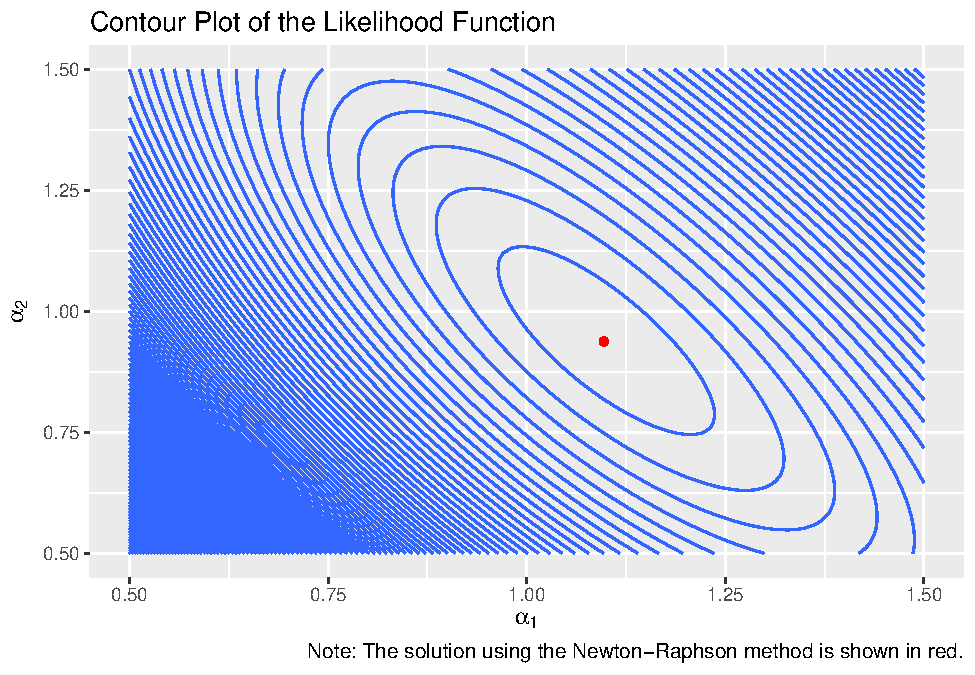
\includegraphics{Atlas-PS_3_files/figure-latex/unnamed-chunk-2-1.pdf}

Next, we implement the Fisher Scoring algorithm.

\begin{Shaded}
\begin{Highlighting}[]
\CommentTok{# We implement the Fisher scoring update method}

\NormalTok{I <-}\StringTok{ }\ControlFlowTok{function}\NormalTok{(alpha, b, x)\{}
  \KeywordTok{return}\NormalTok{(}\KeywordTok{matrix}\NormalTok{(}\KeywordTok{c}\NormalTok{(}
    \KeywordTok{sum}\NormalTok{(b[, }\DecValTok{1}\NormalTok{]}\OperatorTok{^}\DecValTok{2} \OperatorTok{/}\StringTok{ }\NormalTok{(b }\OperatorTok\StringTok{ }\NormalTok{alpha)), }
    \KeywordTok{sum}\NormalTok{(}\KeywordTok{apply}\NormalTok{(b, }\DecValTok{1}\NormalTok{, prod) }\OperatorTok{/}\StringTok{ }\NormalTok{(b }\OperatorTok\StringTok{ }\NormalTok{alpha)),}
    \KeywordTok{sum}\NormalTok{(}\KeywordTok{apply}\NormalTok{(b, }\DecValTok{1}\NormalTok{, prod) }\OperatorTok{/}\StringTok{ }\NormalTok{(b }\OperatorTok\StringTok{ }\NormalTok{alpha)), }
    \KeywordTok{sum}\NormalTok{(b[, }\DecValTok{2}\NormalTok{]}\OperatorTok{^}\DecValTok{2} \OperatorTok{/}\StringTok{ }\NormalTok{(b }\OperatorTok\StringTok{ }\NormalTok{alpha))}
\NormalTok{  ), }\DataTypeTok{ncol=}\DecValTok{2}\NormalTok{))}
\NormalTok{\}}

\NormalTok{fisher_scoring <-}\StringTok{ }\ControlFlowTok{function}\NormalTok{(I, fprime, alpha0, b, x, }\DataTypeTok{max_iter=}\DecValTok{10000}\NormalTok{, }\DataTypeTok{tol=}\NormalTok{.}\DecValTok{001}\NormalTok{)\{}
\NormalTok{  alpha_t <-}\StringTok{ }\NormalTok{alpha0}
  
  \CommentTok{# Iterate through }
  \ControlFlowTok{for}\NormalTok{ (n }\ControlFlowTok{in} \DecValTok{1}\OperatorTok{:}\NormalTok{max_iter)\{}
    \CommentTok{# Set stopping conditions}
    \ControlFlowTok{if}\NormalTok{(}\KeywordTok{sum}\NormalTok{((alpha0 }\OperatorTok{-}\StringTok{ }\NormalTok{alpha_t)}\OperatorTok{^}\DecValTok{2}\NormalTok{) }\OperatorTok{<}\StringTok{ }\NormalTok{tol }\OperatorTok{&}\StringTok{ }\NormalTok{n }\OperatorTok{>}\StringTok{ }\DecValTok{1}\NormalTok{)\{}\ControlFlowTok{break}\NormalTok{\}}
    
\NormalTok{    alpha0 <-}\StringTok{ }\NormalTok{alpha_t}
    
    \CommentTok{# Get the Fisher update}
\NormalTok{    alpha_t <-}\StringTok{ }\NormalTok{alpha0 }\OperatorTok{+}\StringTok{ }\KeywordTok{solve}\NormalTok{(}\KeywordTok{I}\NormalTok{(alpha0, b, x)) }\OperatorTok\StringTok{ }\KeywordTok{fprime}\NormalTok{(alpha0, b, x) }
\NormalTok{  \}}
  
  \KeywordTok{return}\NormalTok{(}\KeywordTok{c}\NormalTok{(}\DataTypeTok{alpha_t=}\NormalTok{alpha_t, }\DataTypeTok{n=}\NormalTok{n))}
\NormalTok{\}}

\CommentTok{# We call the function on our dataset}
\NormalTok{alpha0 <-}\StringTok{ }\KeywordTok{c}\NormalTok{(}\DecValTok{1}\NormalTok{, }\DecValTok{1}\NormalTok{)}
\NormalTok{b <-}\StringTok{ }\KeywordTok{as.matrix}\NormalTok{(oil[, }\KeywordTok{c}\NormalTok{(}\StringTok{'importexport'}\NormalTok{, }\StringTok{'domestic'}\NormalTok{)])}
\NormalTok{x <-}\StringTok{ }\KeywordTok{as.matrix}\NormalTok{(oil[, }\KeywordTok{c}\NormalTok{(}\StringTok{'spills'}\NormalTok{)])}

\NormalTok{solution <-}\StringTok{ }\KeywordTok{fisher_scoring}\NormalTok{(}\DataTypeTok{I=}\NormalTok{I, }\DataTypeTok{fprime=}\NormalTok{fprime, }\DataTypeTok{alpha0=}\KeywordTok{c}\NormalTok{(}\DecValTok{1}\NormalTok{, }\DecValTok{1}\NormalTok{), }\DataTypeTok{b=}\NormalTok{b, }\DataTypeTok{x=}\NormalTok{x, }\DataTypeTok{tol=}\NormalTok{.}\DecValTok{00001}\NormalTok{)}
\end{Highlighting}
\end{Shaded}

The solution is given as \(\alpha = [1.097, .938]\), converging in 6
iterations. Below, the contour plot for the likelihood function is
shown, with the green dot labelling the given solution. We see that the
algorithm appears to have converged on the solution. Note that this is
the same solution seen above with Newton's Algorithm. This is as
expected, as the two techniques are quite similar.

\begin{Shaded}
\begin{Highlighting}[]
\NormalTok{log_likelihood <-}\StringTok{ }\ControlFlowTok{function}\NormalTok{(alpha, b, x)\{}
  \KeywordTok{return}\NormalTok{(}\KeywordTok{sum}\NormalTok{(x }\OperatorTok{*}\StringTok{ }\KeywordTok{log}\NormalTok{(b }\OperatorTok\StringTok{ }\NormalTok{alpha)) }\OperatorTok{-}\StringTok{ }\KeywordTok{sum}\NormalTok{(alpha[}\DecValTok{1}\NormalTok{] }\OperatorTok{*}\StringTok{ }\NormalTok{b[, }\DecValTok{1}\NormalTok{]) }
         \OperatorTok{-}\StringTok{ }\KeywordTok{sum}\NormalTok{(alpha[}\DecValTok{2}\NormalTok{] }\OperatorTok{*}\StringTok{ }\NormalTok{b[, }\DecValTok{2}\NormalTok{]) }\OperatorTok{-}\StringTok{ }\KeywordTok{sum}\NormalTok{(}\KeywordTok{log}\NormalTok{(}\KeywordTok{factorial}\NormalTok{(x))))}
\NormalTok{\}}

\CommentTok{# we construct agrid of the likelihood function to plot the contours}
\NormalTok{a1 <-}\StringTok{ }\KeywordTok{seq}\NormalTok{(}\FloatTok{0.1}\NormalTok{, }\DecValTok{2}\NormalTok{, .}\DecValTok{01}\NormalTok{)}
\NormalTok{a2 <-}\StringTok{ }\KeywordTok{seq}\NormalTok{(}\FloatTok{0.1}\NormalTok{, }\DecValTok{2}\NormalTok{, .}\DecValTok{01}\NormalTok{)}
\NormalTok{alpha_space <-}\StringTok{ }\KeywordTok{as.matrix}\NormalTok{(}\KeywordTok{expand.grid}\NormalTok{(a1, a2)) }\CommentTok{# Create cartesian product}

\CommentTok{# Find the likelihod for all pairs}
\NormalTok{results <-}\StringTok{ }\KeywordTok{data.frame}\NormalTok{(}\KeywordTok{cbind}\NormalTok{(}
\NormalTok{  alpha_space, }\KeywordTok{apply}\NormalTok{(}
\NormalTok{    alpha_space, }\DecValTok{1}\NormalTok{, }
      \ControlFlowTok{function}\NormalTok{(alpha) }\KeywordTok{log_likelihood}\NormalTok{(alpha, }\DataTypeTok{b=}\NormalTok{b, }\DataTypeTok{x=}\NormalTok{x))))}

\CommentTok{# Add column names}
\KeywordTok{colnames}\NormalTok{(results) <-}\StringTok{ }\KeywordTok{c}\NormalTok{(}\StringTok{"alpha1"}\NormalTok{, }\StringTok{"alpha2"}\NormalTok{, }\StringTok{"likelihood"}\NormalTok{) }

\CommentTok{# Plot the contours with the solution in red}
\KeywordTok{ggplot}\NormalTok{(results) }\OperatorTok{+}\StringTok{ }
\StringTok{  }\KeywordTok{geom_contour}\NormalTok{(}\KeywordTok{aes}\NormalTok{(}\DataTypeTok{x=}\NormalTok{alpha1, }\DataTypeTok{y=}\NormalTok{alpha2, }\DataTypeTok{z=}\NormalTok{likelihood), }\DataTypeTok{bins=}\DecValTok{1000}\NormalTok{) }\OperatorTok{+}\StringTok{ }
\StringTok{  }\KeywordTok{geom_point}\NormalTok{(}\KeywordTok{aes}\NormalTok{(}\DataTypeTok{x=}\NormalTok{solution[}\DecValTok{1}\NormalTok{], }\DataTypeTok{y=}\NormalTok{solution[}\DecValTok{2}\NormalTok{]), }\DataTypeTok{colour=}\StringTok{"green"}\NormalTok{) }\OperatorTok{+}
\StringTok{  }\KeywordTok{xlab}\NormalTok{(}\KeywordTok{TeX}\NormalTok{(}\StringTok{"$}\CharTok{\textbackslash{}\textbackslash{}}\StringTok{alpha_1$"}\NormalTok{)) }\OperatorTok{+}\StringTok{ }\KeywordTok{ylab}\NormalTok{(}\KeywordTok{TeX}\NormalTok{(}\StringTok{"$}\CharTok{\textbackslash{}\textbackslash{}}\StringTok{alpha_2$"}\NormalTok{)) }\OperatorTok{+}\StringTok{ }
\StringTok{  }\KeywordTok{ggtitle}\NormalTok{(}\StringTok{"Contour Plot of the Likelihood Function"}\NormalTok{) }\OperatorTok{+}
\StringTok{  }\KeywordTok{labs}\NormalTok{(}\DataTypeTok{caption=}\StringTok{"Note: The solution using Fisher Scoring is shown in green."}\NormalTok{)}
\end{Highlighting}
\end{Shaded}

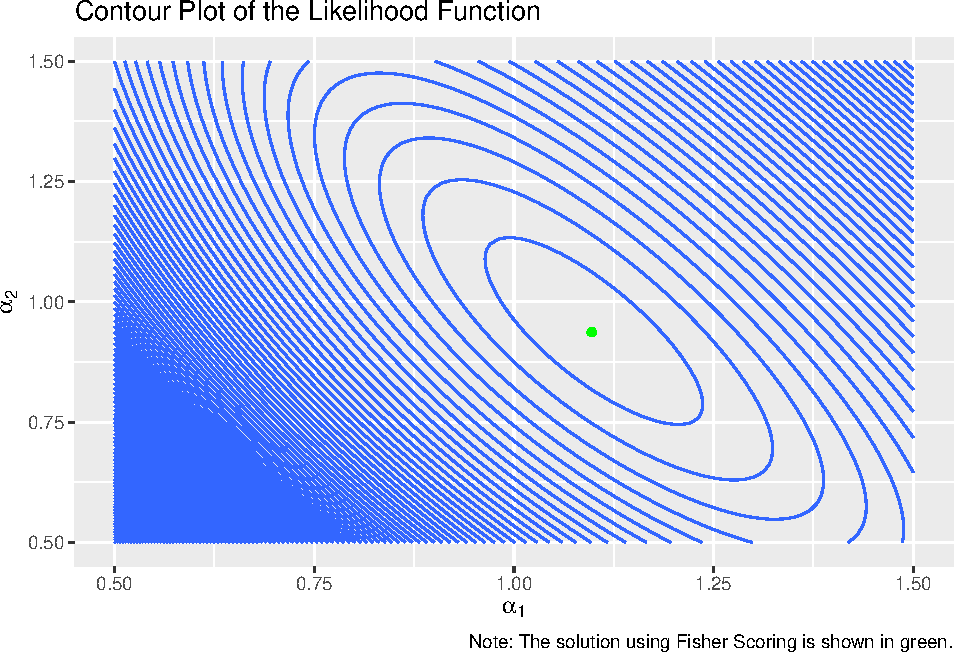
\includegraphics{Atlas-PS_3_files/figure-latex/unnamed-chunk-4-1.pdf}


\end{document}
